% Required packages: graphicx, rotating
% Adjust the path prefix if this file is copied outside the project root.
\begin{sidewaysfigure}[p]
\centering
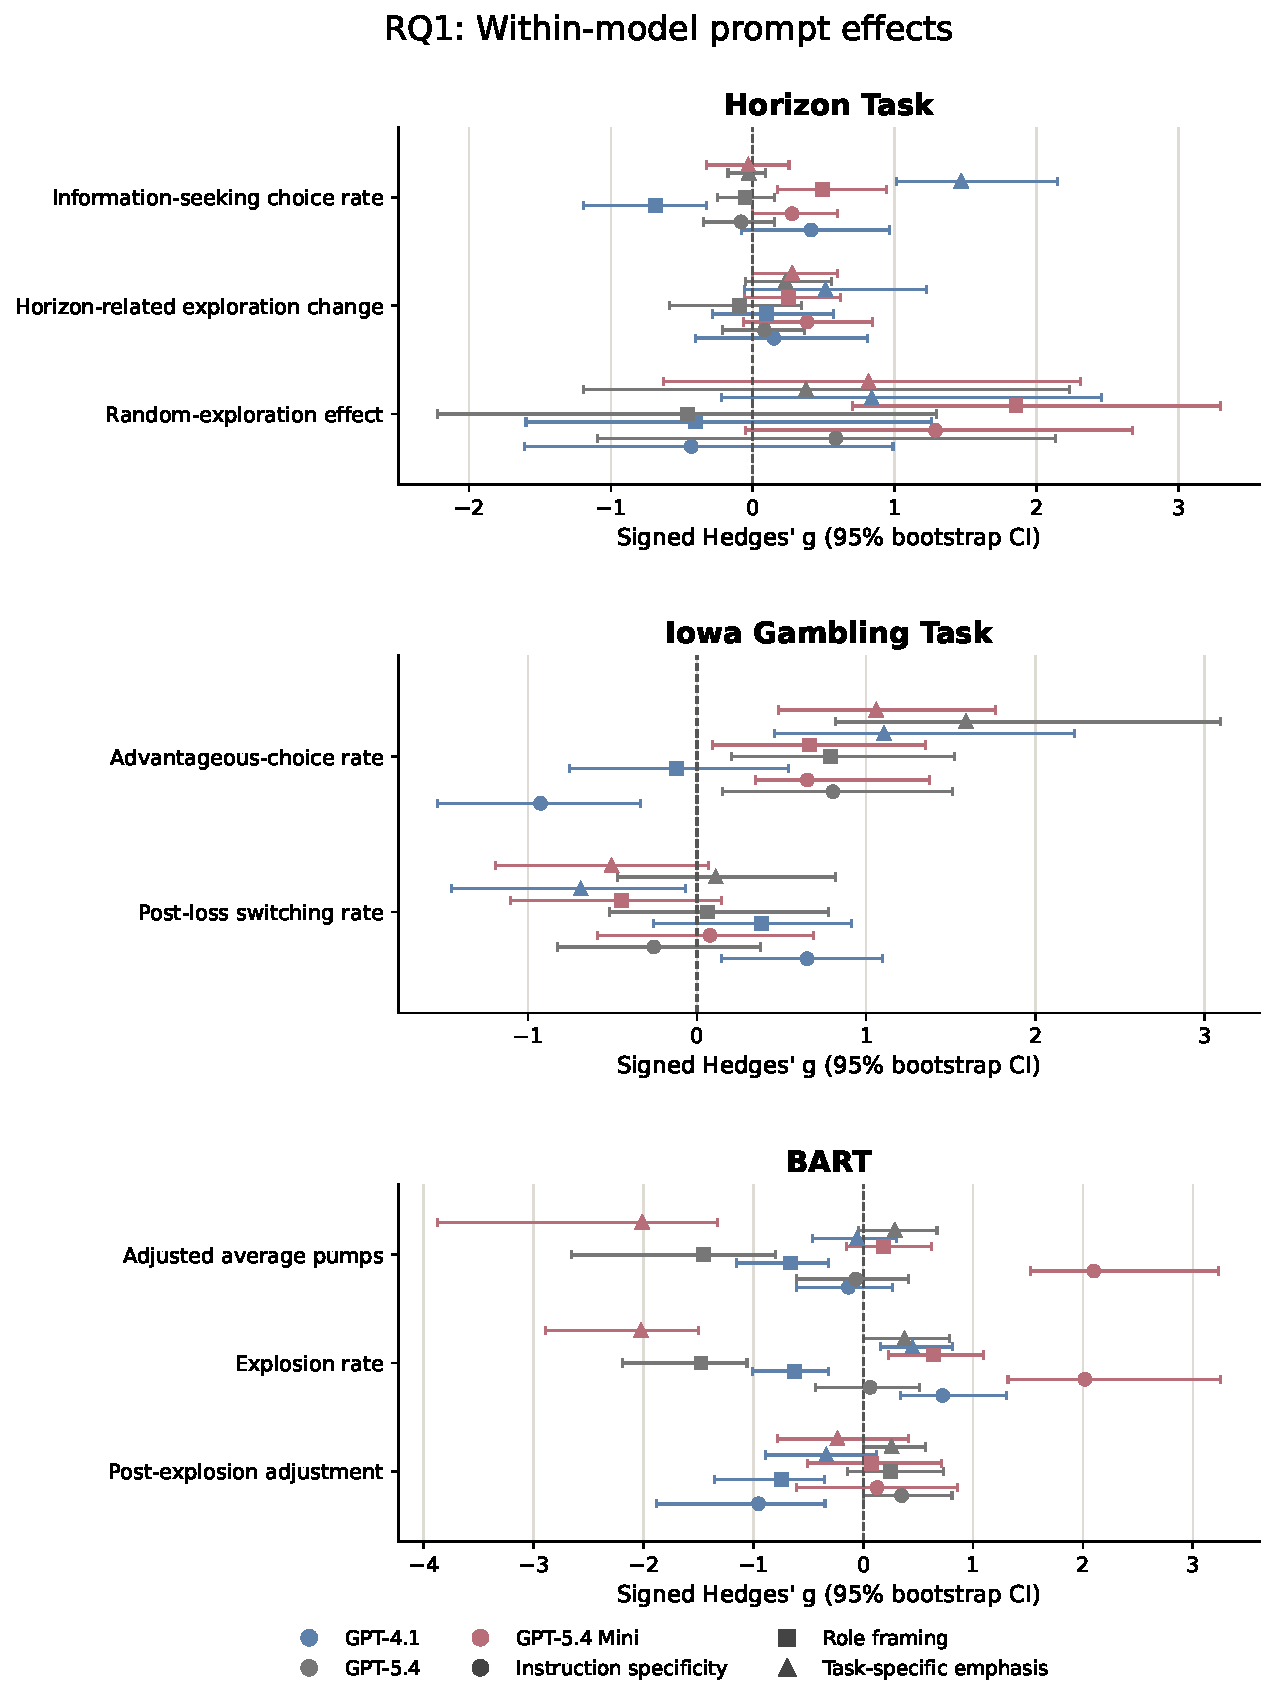
\includegraphics[width=\textheight]{outputs/figures/final_results_v01/figure_rq1_prompt_effects_overview.pdf}
\caption{Task-grouped forest plots of within-model prompt effects relative to Neutral (RQ1). Horizon, IGT, and BART are arranged as three horizontal panels. Points are signed Hedges' $g$ estimates and horizontal lines are percentile-bootstrap 95\% confidence intervals; colour and shape identify model. Raw effects, raw confidence intervals, and PSI are reported in the supplementary tables.}
\label{fig:rq1}
\end{sidewaysfigure}

\begin{sidewaysfigure}[p]
\centering
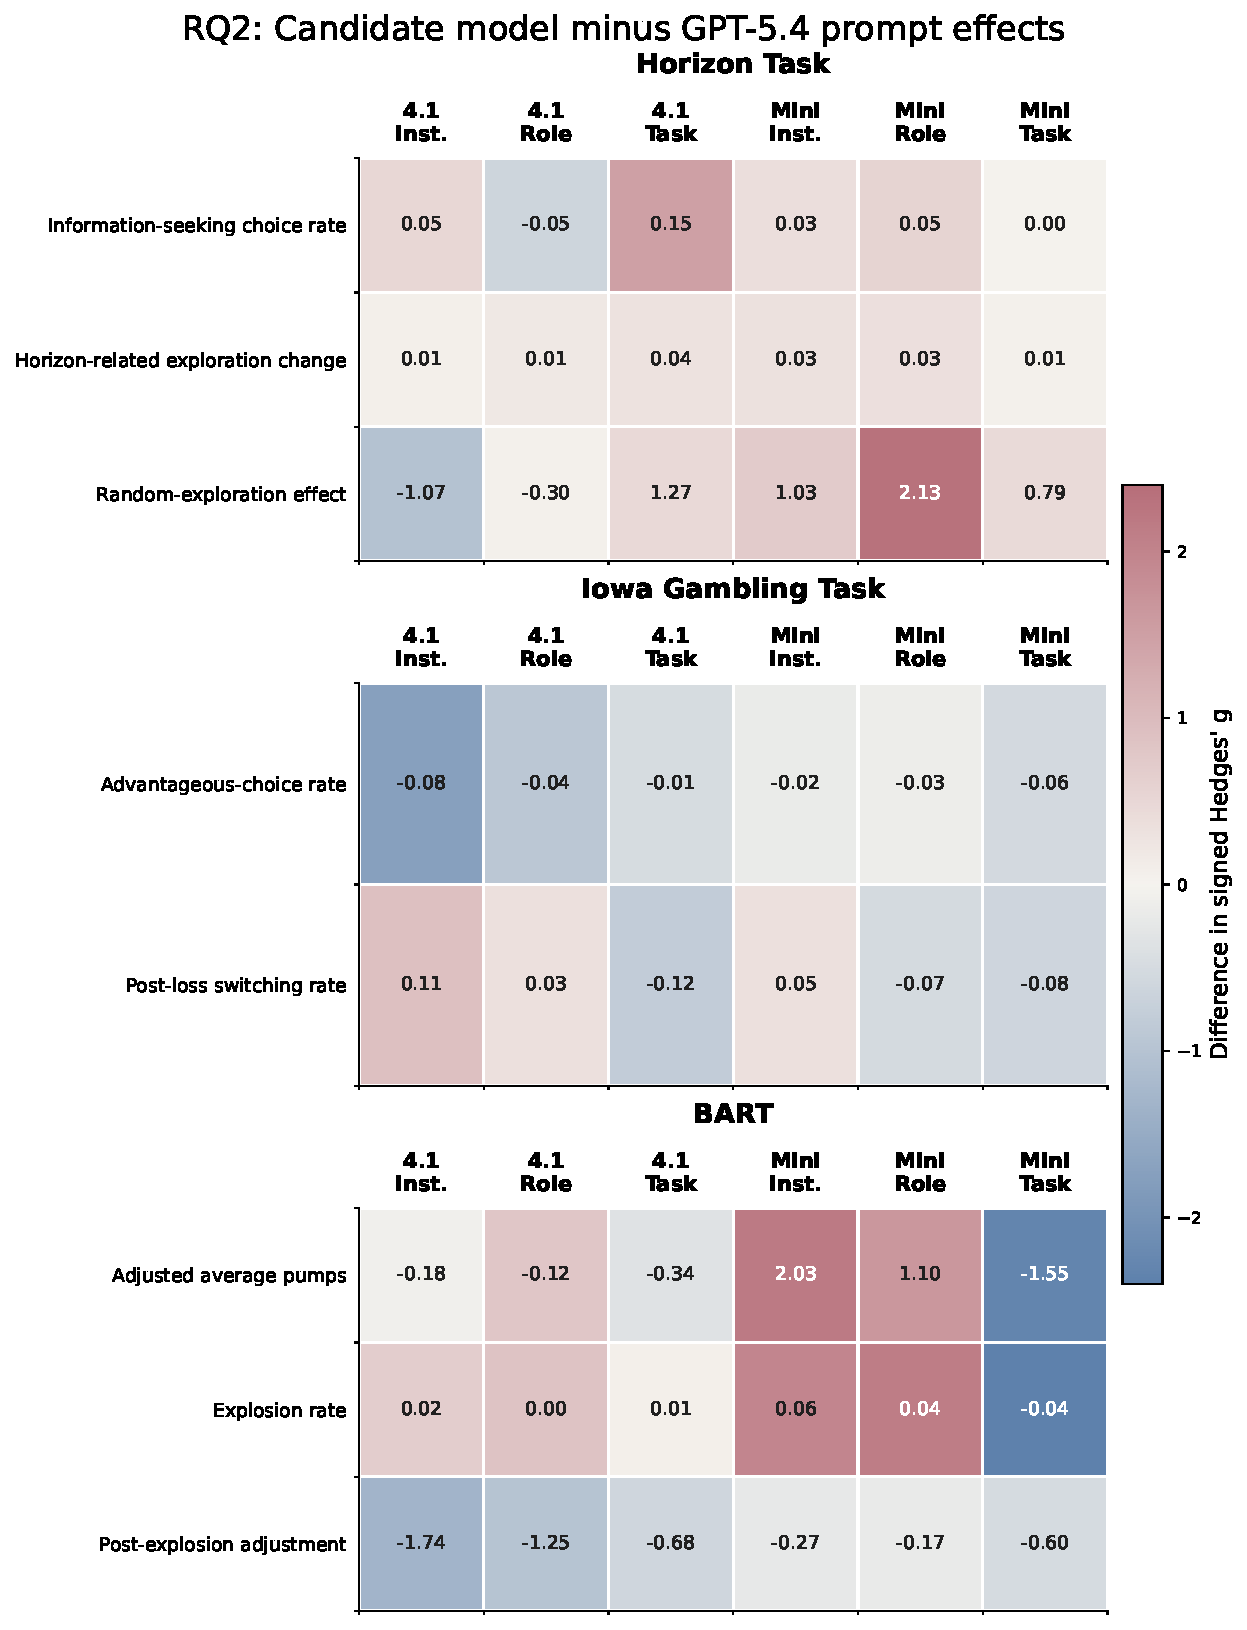
\includegraphics[width=\textheight]{outputs/figures/final_results_v01/figure_rq2_model_interactions_overview.pdf}
\caption{Task-grouped overview of model-by-prompt interaction contrasts (RQ2). Horizon, IGT, and BART are arranged as three horizontal panels. Cell text is the raw interaction $(\bar{Y}_{\mathrm{target},p}-\bar{Y}_{\mathrm{target},N})-(\bar{Y}_{\mathrm{GPT\text{-}5.4},p}-\bar{Y}_{\mathrm{GPT\text{-}5.4,N})$. Colour is the descriptive difference between the two models' signed Hedges' $g$ values. Raw percentile-bootstrap 95\% confidence intervals are reported in the supplementary table; the complete metric-specific forest display is retained in the appendix package.}
\label{fig:rq2}
\end{sidewaysfigure}

\begin{sidewaysfigure}[p]
\centering
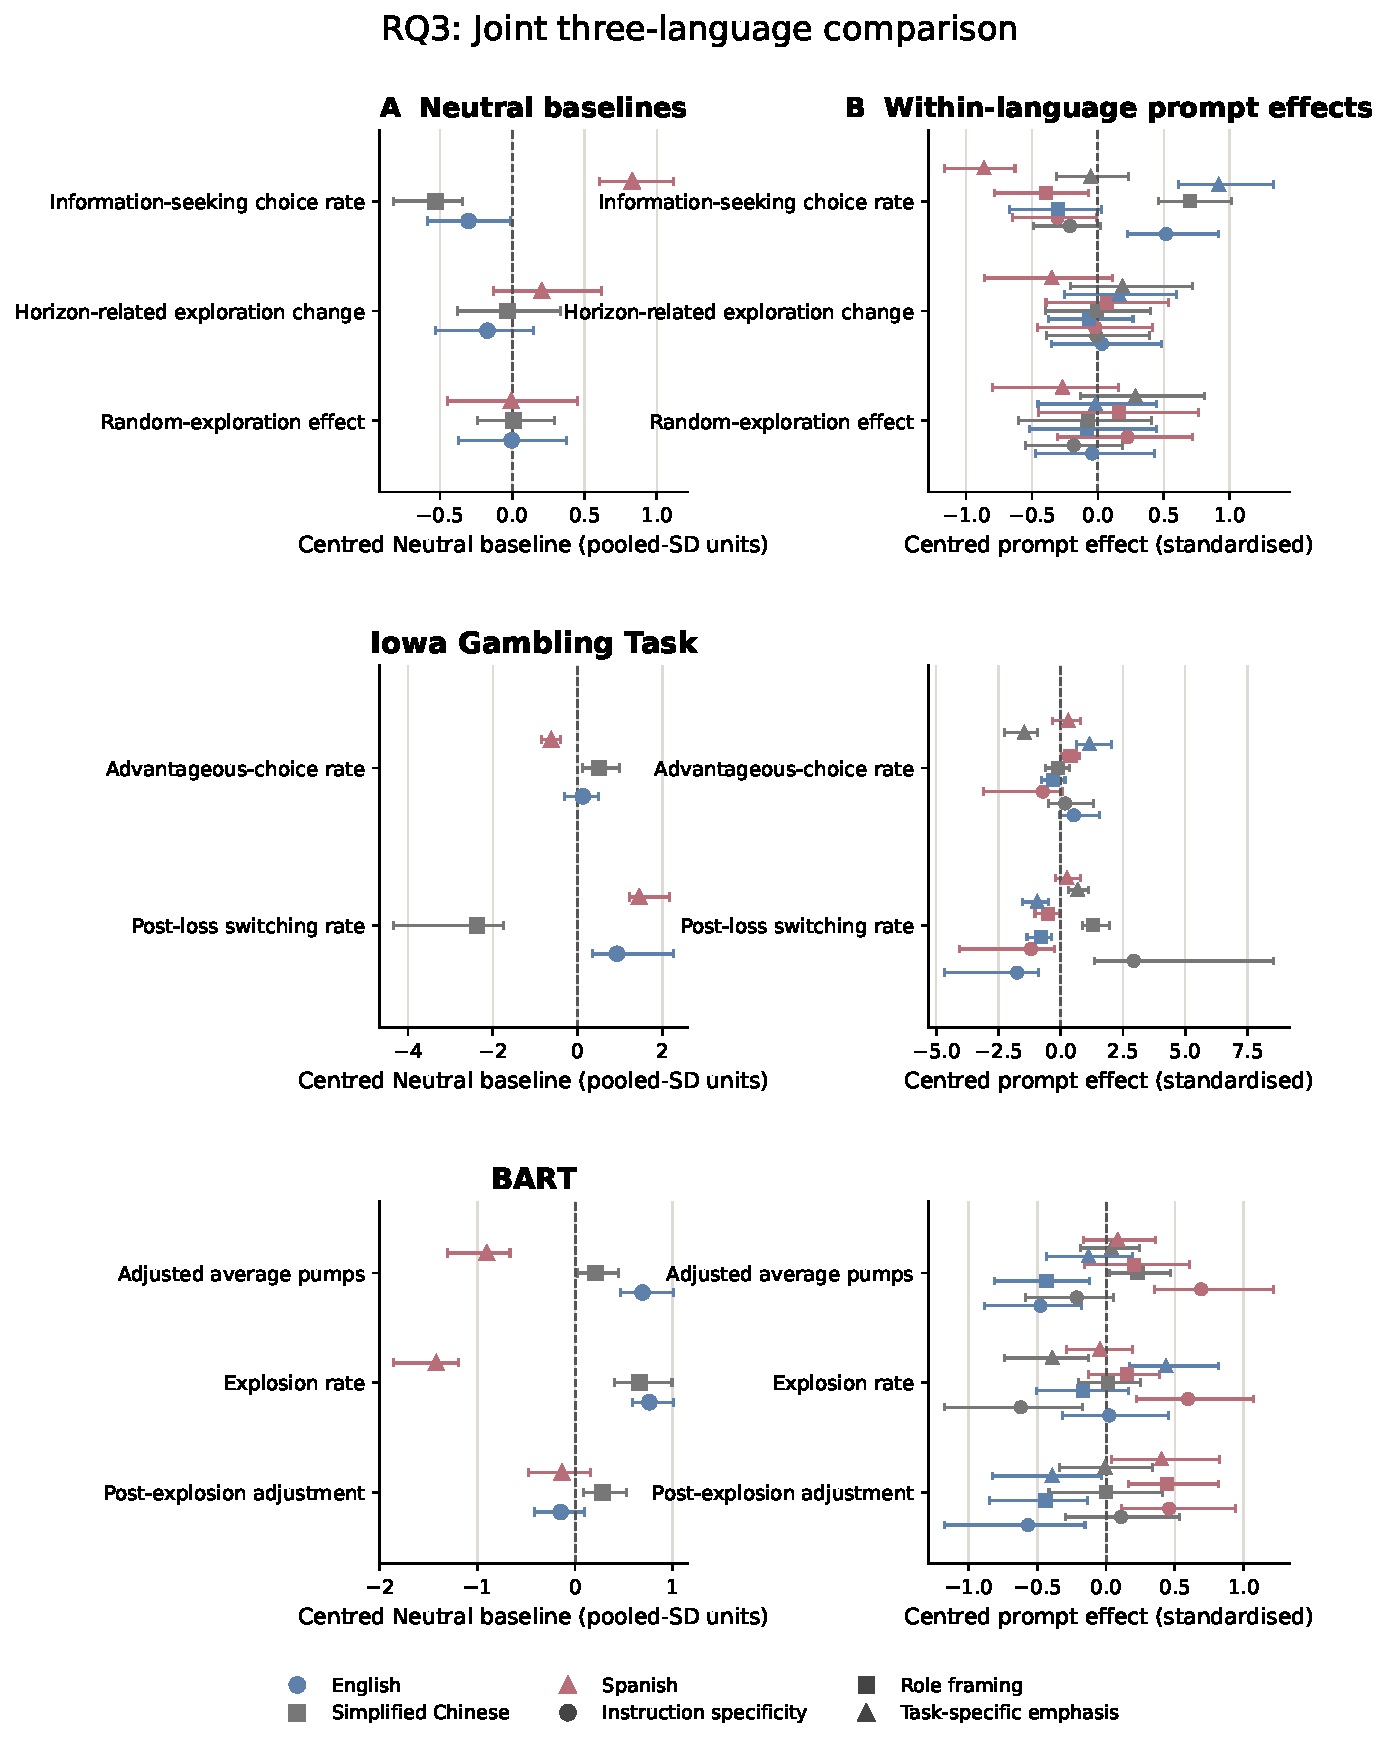
\includegraphics[width=\textheight]{outputs/figures/final_results_v01/figure_rq3_language_overview.pdf}
\caption{Task-grouped forest plots for the joint GPT-4.1 three-language comparison (RQ3). Columns distinguish Horizon, IGT, and BART. The upper row plots each language's Neutral mean deviation from the three-language mean, scaled by the pooled within-language run SD. The lower row plots each language's Hedges' $g$ minus the corresponding three-language mean Hedges' $g$. Both rows include percentile-bootstrap 95\% confidence intervals; the three language-specific deviations sum to zero within each comparison, so no language is designated as a reference. Raw centred estimates and intervals are reported in the supplementary tables.}
\label{fig:rq3}
\end{sidewaysfigure}

\begin{sidewaysfigure}[p]
\centering
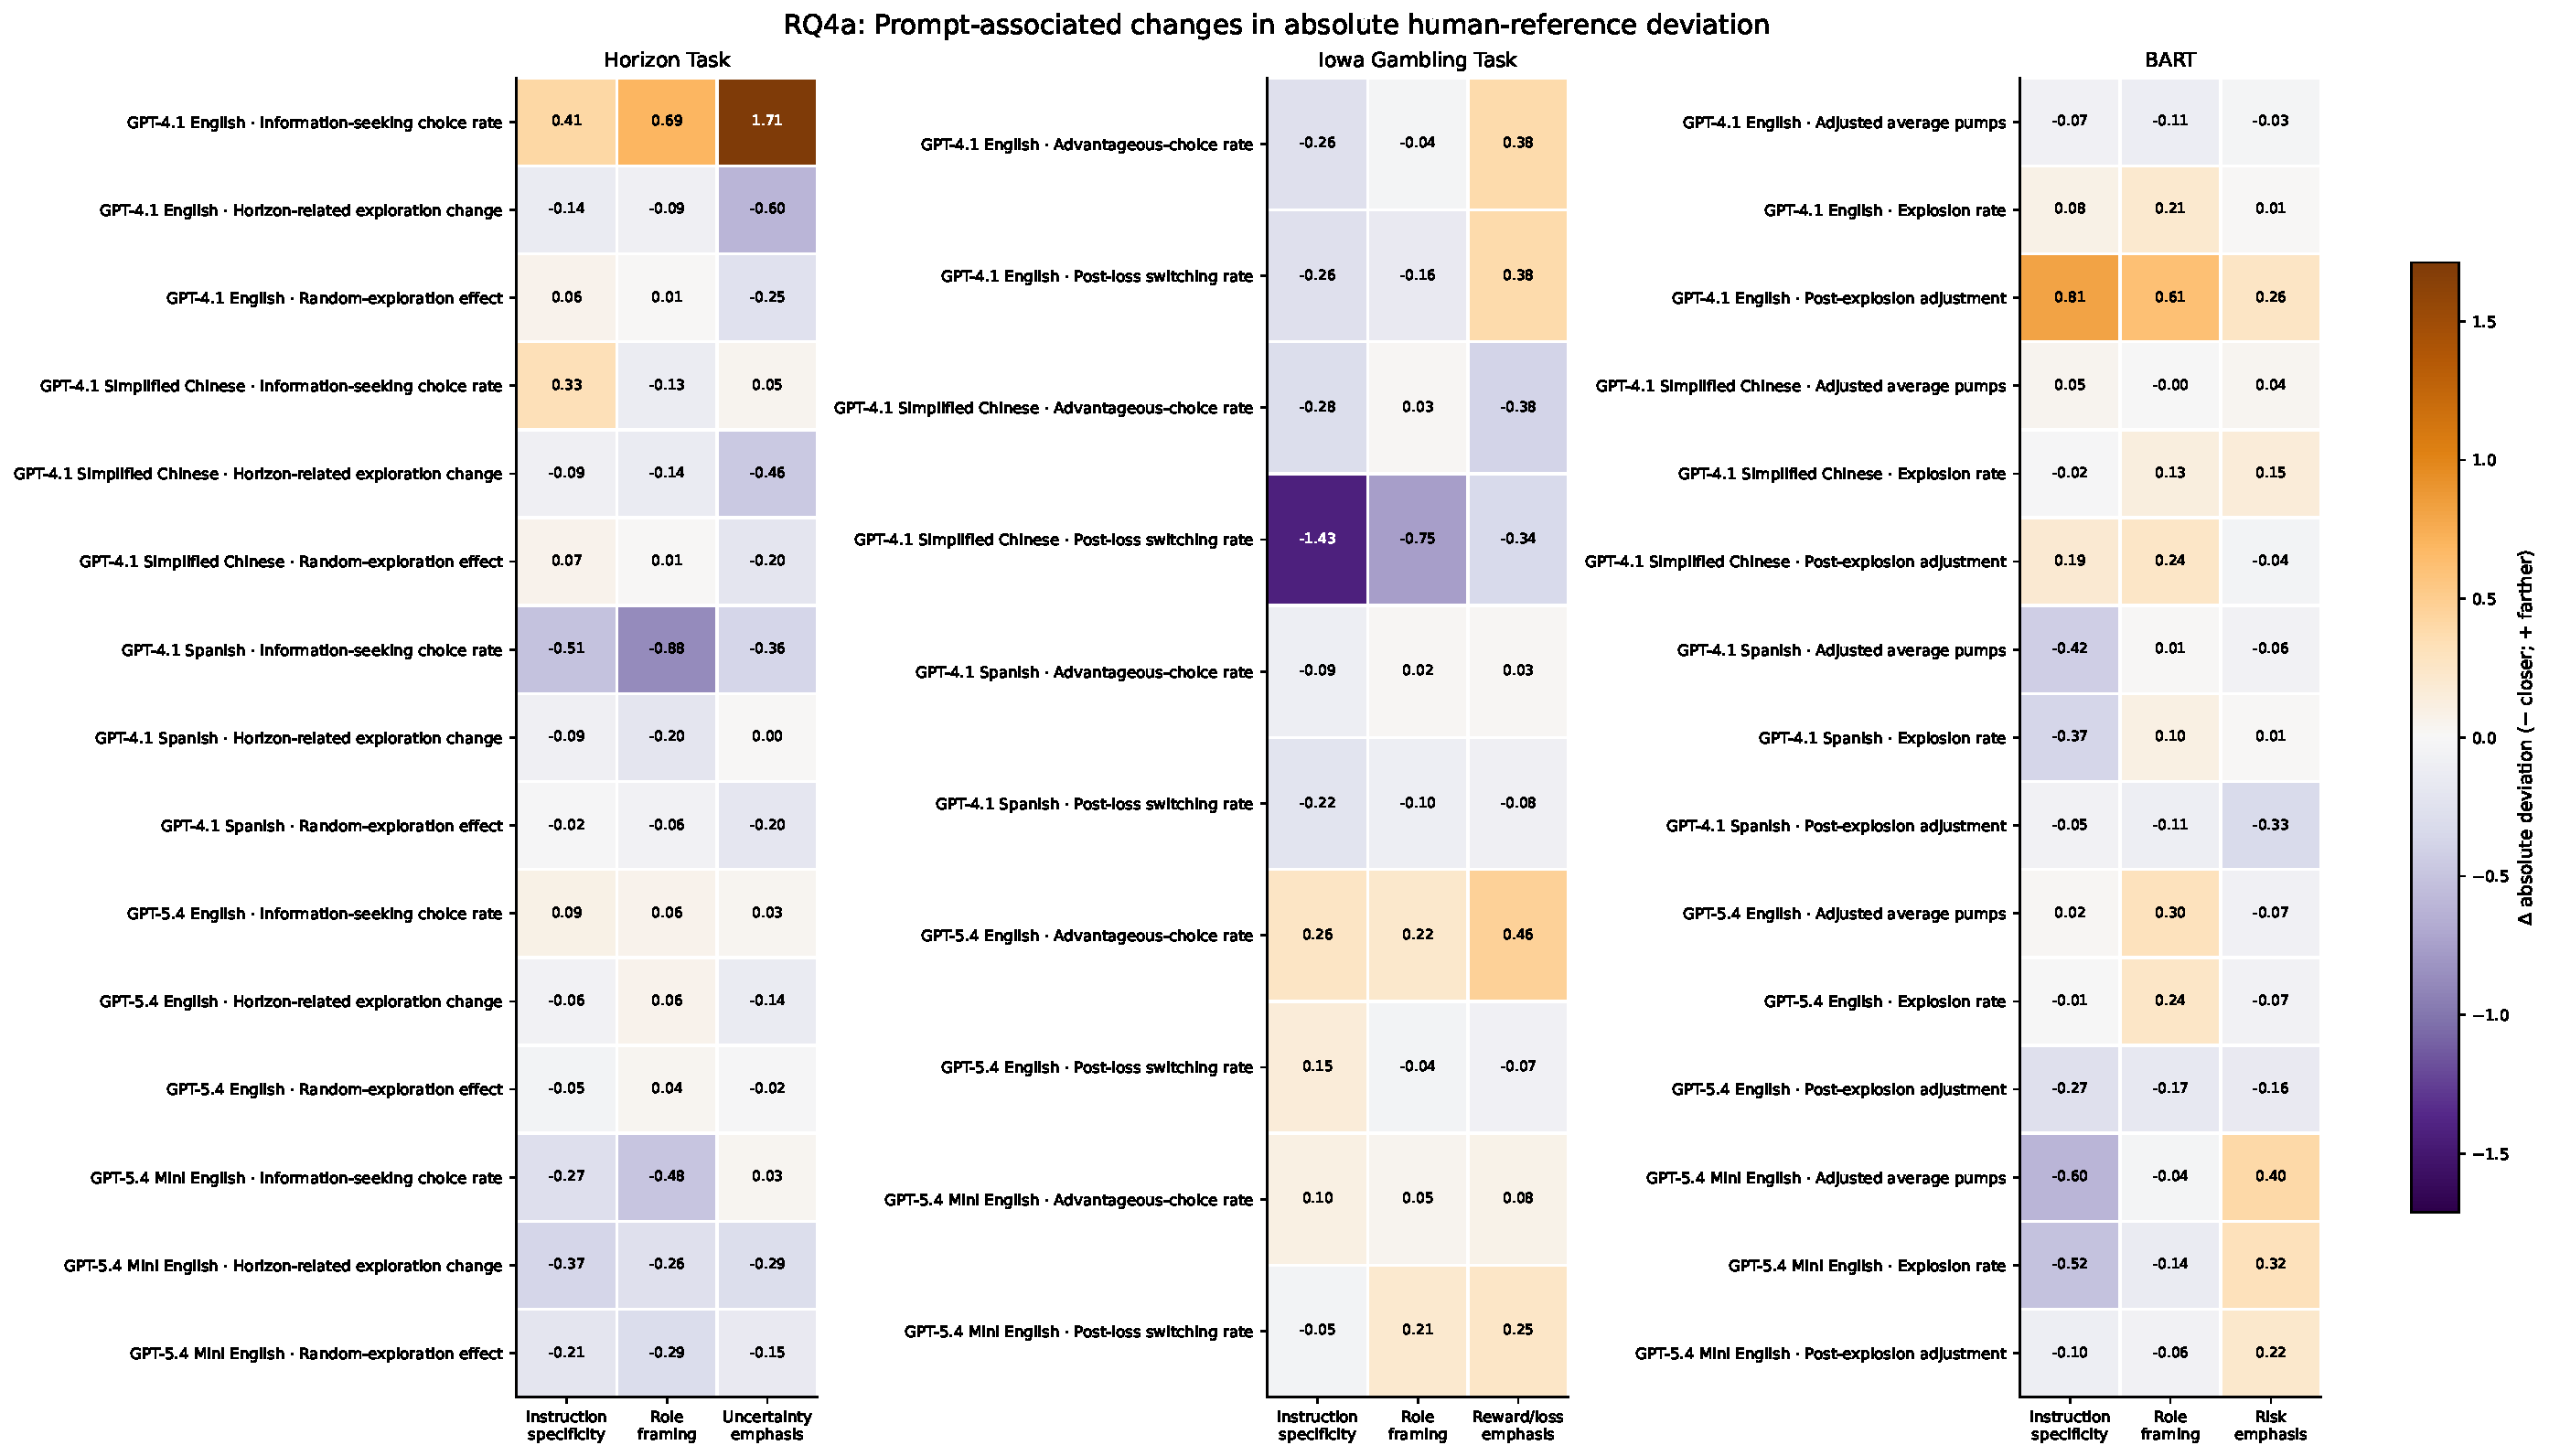
\includegraphics[width=\textheight]{outputs/figures/final_results_v01/figure_rq4_absolute_deviation_heatmap.pdf}
\caption{Prompt-associated changes in absolute human-SD-scaled mean deviation (RQ4a). Cells contain descriptive point-estimated manipulated-minus-Neutral changes: negative values indicate movement closer to the human mean and positive values movement farther away. No inferential intervals were constructed for these human-reference proximity measures.}
\label{fig:rq4a}
\end{sidewaysfigure}

\begin{sidewaysfigure}[p]
\centering
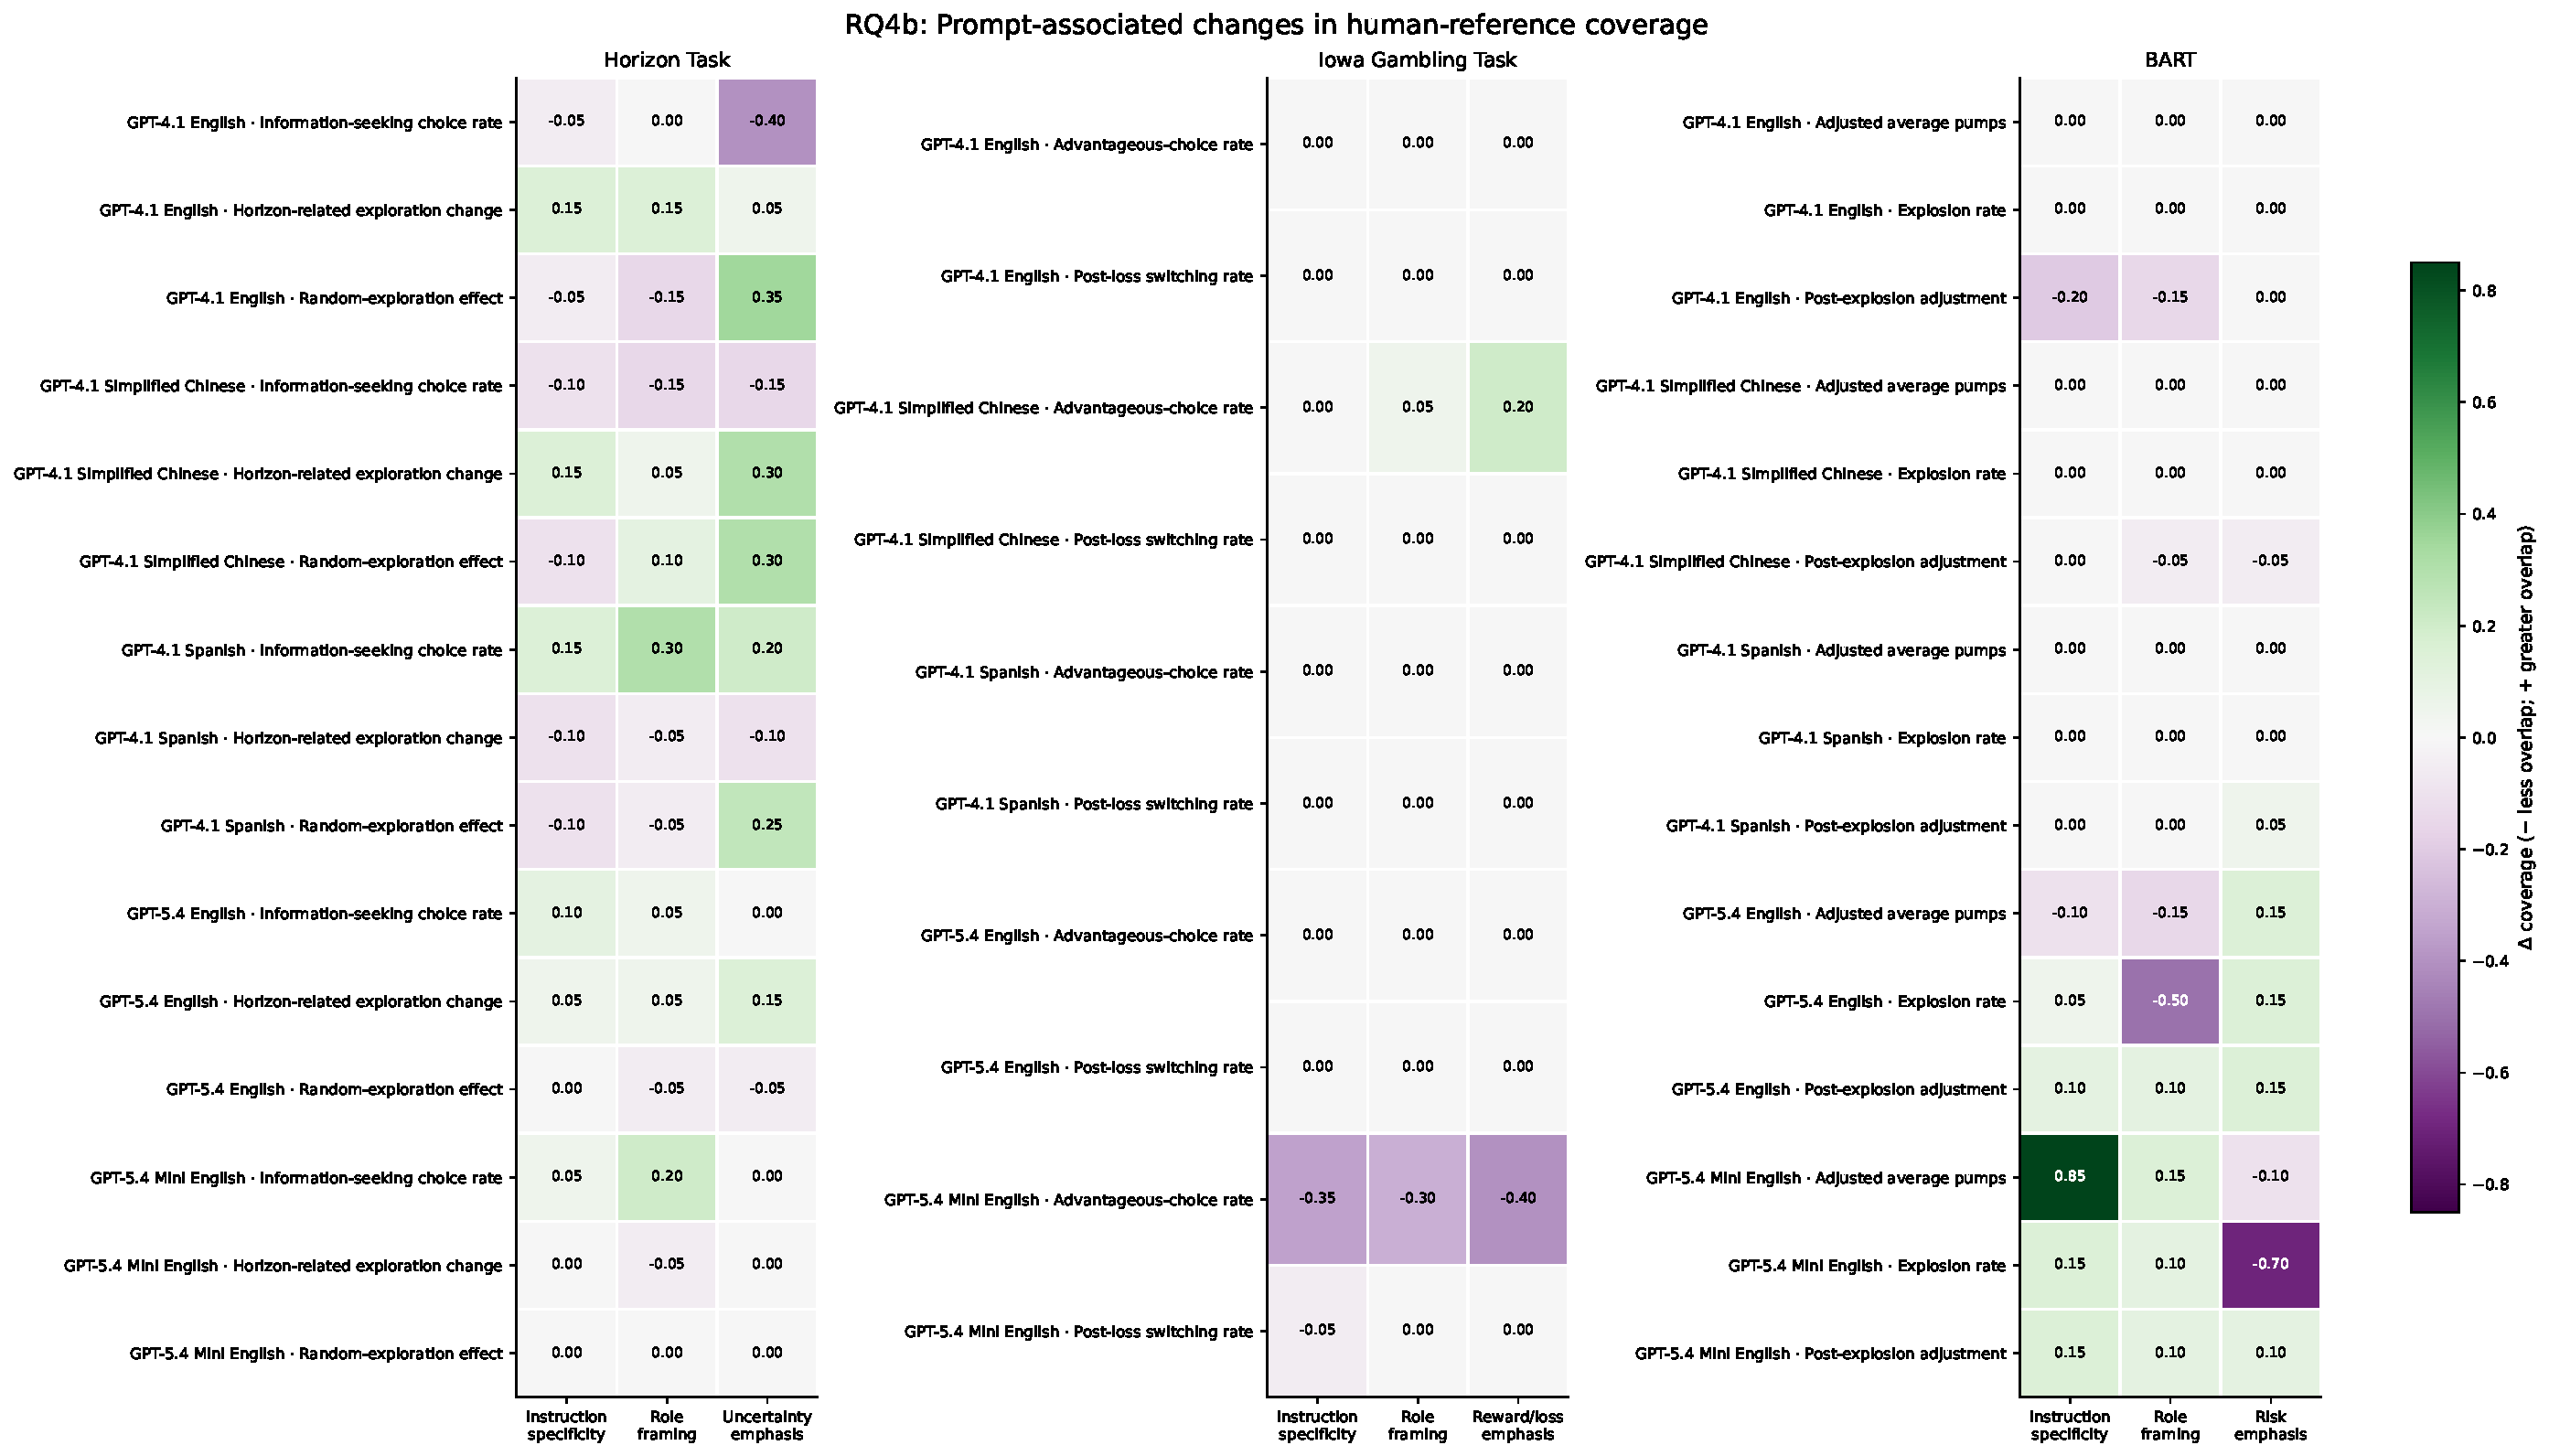
\includegraphics[width=\textheight]{outputs/figures/final_results_v01/figure_rq4_coverage_heatmap.pdf}
\caption{Prompt-associated changes in empirical human-reference coverage (RQ4b). Cells contain descriptive point-estimated manipulated-minus-Neutral changes: positive values indicate greater overlap with the empirical human range and negative values less overlap. Coverage is quantised by the valid-run denominator (in increments of 0.05 when all 20 runs are non-missing). No inferential intervals were constructed for these human-reference proximity measures; neither RQ4 display is an equivalence test or evidence of a shared mechanism.}
\label{fig:rq4b}
\end{sidewaysfigure}
